% Compile with: latexmk -pdf II2202-research-plan-slides.tex
\documentclass[aspectratio=169,11pt]{beamer}

\usepackage[T1]{fontenc}
\usepackage{lmodern}
\usepackage{booktabs}
\usepackage{graphicx}
\usepackage{xcolor}

\definecolor{ink}{HTML}{111111}
\definecolor{quiet}{HTML}{555555}

\usetheme{default}
\usecolortheme{default}
\setbeamertemplate{navigation symbols}{}
\setbeamertemplate{headline}{}
\setbeamercolor{background canvas}{bg=white}
\setbeamercolor{normal text}{fg=ink}
\setbeamercolor{frametitle}{fg=ink}
\setbeamercolor{title}{fg=ink}
\setbeamercolor{author}{fg=ink}
\setbeamercolor{institute}{fg=quiet}
\setbeamercolor{date}{fg=quiet}
\setbeamercolor{structure}{fg=ink}
\setbeamerfont{frametitle}{size=\large,series=\bfseries}
\setbeamerfont{title}{size=\Large,series=\bfseries}
\setbeamerfont{author}{size=\normalsize}
\setbeamerfont{institute}{size=\small}
\setbeamerfont{date}{size=\small}

\setbeamersize{text margin left=1.05cm,text margin right=1.05cm}

\setbeamertemplate{frametitle}{%
  \vspace{0.2cm}%
  {\usebeamerfont{frametitle}\insertframetitle\par}%
  \vspace{0.12cm}%
  {\color{ink}\hrule height 0.35pt}%
  \vspace{0.28cm}%
}

\setbeamertemplate{footline}{%
  \vspace{0.08cm}%
  \hspace{1.05cm}{\scriptsize\color{quiet}II2202 · Research plan}%
  \hfill
  {\scriptsize\color{quiet}\insertframenumber/\inserttotalframenumber}\hspace{1.05cm}%
  \vspace{0.2cm}%
}

\setbeamertemplate{itemize item}{--}
\setlength{\leftmargini}{1.05em}

\title{Transparent Multi-Hop Routing for Raft\\under Partial Network Partitions}
\author{Lorenzo Deflorian \and Juozas Skarbalius}
\institute{KTH \\II2202 Research Methodology and Scientific Writing}
\date{September 2026}

\begin{document}

% ------------------------------------------------------------
\begin{frame}[plain]
  \vspace{1.4cm}
  {\usebeamerfont{title}\inserttitle\par}
  \vspace{0.75em}
  {\normalsize Lorenzo Deflorian \textless ldef@kth.se\textgreater\par}
  {\normalsize Juozas Skarbalius \textless juozas@kth.se\textgreater\par}
  \vspace{0.9em}
  {\small\color{quiet}KTH\par}
  {\small\color{quiet}II2202 Research Methodology and Scientific Writing\par}
  \vspace{0.35em}
  {\small\color{quiet}September 2026\par}
\end{frame}

% ------------------------------------------------------------
\begin{frame}[t,shrink=5]{Research topic and problem}
\textbf{Problem.}
In Raft, leader needs majority quorum. Under certain partial partitions, this quorum could not be stabely maintained. 
Overlay routing is proposed by prior work, but significantly not tested with Raft.

\smallskip
\textbf{RQ1.} In which partial partitions does forwarding restore stable progress?\\
\textbf{RQ2.} How does added hop delay change commit latency?

\vspace{0.3em}
\begin{center}
  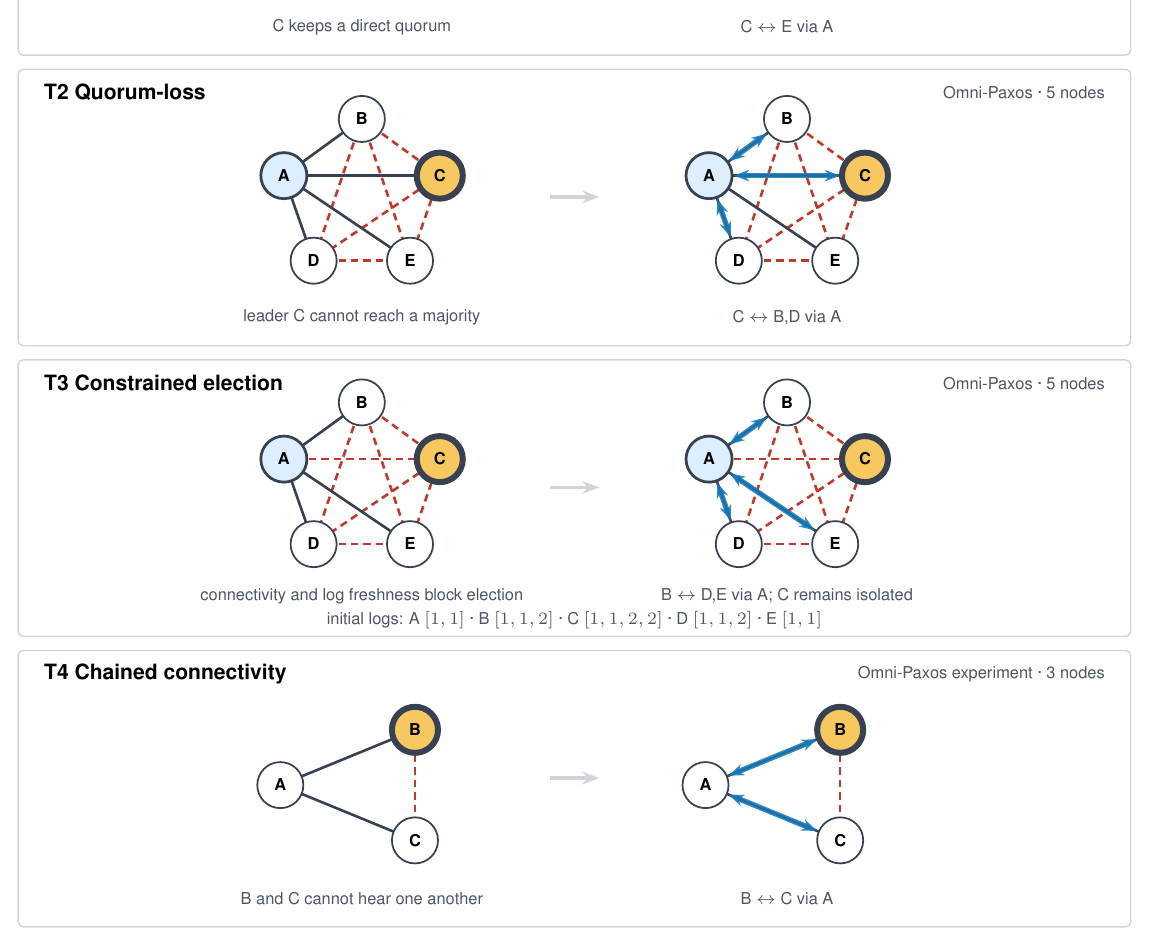
\includegraphics[width=\textwidth,height=2.95cm,keepaspectratio]{topology-excerpt.png}\\[0.08em]
  {\scriptsize\color{quiet}Excerpt of planned topologies (direct vs.\ transparent forwarding)}
\end{center}
\end{frame}

% ------------------------------------------------------------
\begin{frame}{Research method and work plan}
  \begin{columns}[T,onlytextwidth]
    \begin{column}{0.55\textwidth}
      \textbf{Experimental method}\\[0.35em]
      {\footnotesize
      \begin{itemize}\itemsep0.28em
        \item HashiCorp Raft implementation
        \item Preconfigured network forwarding using Mininet.
        \item Open-loop client; repeated trials
      \end{itemize}}

      \vspace{0.55em}
      {\footnotesize
      \begin{tabular}{@{}p{2.6cm}p{4.4cm}@{}}
        \toprule
        Factor & Levels \\
        \midrule
        Communication & P2P RPC; multi-hop forwarding \\
        Topology & T0--T4 \\
        Per-link delay & 0.5, 5, 20\,ms \\
        \bottomrule
      \end{tabular}}

      \vspace{0.45em}
      {\scriptsize\color{quiet}Measured: commit progress, recovery time, elections, commit latency}
    \end{column}
    \begin{column}{0.40\textwidth}
      \textbf{Work plan}\\[0.35em]
      {\footnotesize
      \begin{enumerate}\itemsep0.38em
        \item Build Raft + Mininet experiment environment
        \item Pilot runs (5 per condition) for verification
        \item Run all topologies for multiple repetitions ($R=20$)
        \item Data collection and analysis
        \item Write report
      \end{enumerate}}

      \vspace{0.7em}
      {\scriptsize\color{quiet}
      Lorenzo --- Raft, client, RQ1\\[0.15em]
      Juozas --- network, delays, RQ2}
    \end{column}
  \end{columns}
\end{frame}

% ------------------------------------------------------------
\begin{frame}{Key ethical issues}
  \begin{columns}[T,onlytextwidth]
    \begin{column}{0.48\textwidth}
      {\footnotesize
      \textbf{Human Participants and Data}\\[0.5em]
      \begin{itemize}\itemsep0.2em
        \item No human participants
        \item No collection of sensitive or personal data
        \item Open-source software only
      \end{itemize}

      \textbf{Integrity}\\[0.5em]
      \begin{itemize}\itemsep0.2em
        \item Deterministic experiment setup
        \item Report negative findings as results
        \item AI tools may be used for assistence but not for intelectual work
      \end{itemize}}
    \end{column}
  \end{columns}
\end{frame}

% ------------------------------------------------------------
\begin{frame}{Key sustainability issues}
  \begin{columns}[T,onlytextwidth]
    \begin{column}{0.45\textwidth}
      {\footnotesize
      \textbf{Environmental}\\[0.3em]
      \begin{itemize}\itemsep0.25em
        \item In our experiment: local VMs, not cloud infra
        \item Run pilot experiments before full benchmarks
        \item Negative higher level: network overlays might induce higher computing/network consumption.
        \item Positive higher level: proven resilience --> more efficient use of resources.
      \end{itemize}}
    \end{column}
    \begin{column}{0.45\textwidth}
      {\footnotesize
      \textbf{Economic}\\[0.3em]
      \begin{itemize}\itemsep0.25em
        \item In our experiment: our own hardware only
        \item Higher level (negative): infrastructure costs might be higher
        \item Higher level (positive): proven resilience --> more efficient use of resources.
      \end{itemize}}
    \end{column}
  \end{columns}

  \vspace{0.9em}
  {\footnotesize
  \textbf{Relevance.}
  Knowing when multi-hop routing restores progress may reduce prolonged stalls
  and redundant failover under partial partitions.}
\end{frame}

\end{document}
